\documentclass[border=1mm]{standalone}
% \documentclass{article}
\usepackage[margin=2.5cm]{geometry}

\usepackage{graphicx,tikz,tikz-layers,amsmath} 
\usetikzlibrary{decorations.markings,calc,positioning,arrows,shapes.geometric,arrows.meta,3d}

\colorlet{myred}{red!80!black}
\colorlet{myblue}{blue!80!black}
\colorlet{mybluee}{myblue!80!black}
\colorlet{mygreen}{green!60!black}
\colorlet{myorange}{orange!70!red!60!black}
\colorlet{mydarkred}{red!20!black}
\colorlet{mydarkblue}{blue!40!black}
\colorlet{mydarkgreen}{green!20!black}




\begin{document}

\resizebox{.9\textwidth}{!}{
\tikz[font=\footnotesize,scale=1, every node/.style={outer sep=0pt, inner sep=0pt,align=center}, w/.style={minimum width=#1},h/.style={minimum height=#1},s/.style={minimum size=#1}, eu/.style={shorten >=#1},ed/.style={shorten <=#1}, line join=round]
{
\tikzset{>={Latex[length=1.75mm,width=1.25mm]}}
% \tikzset{>={Latex[length=2mm,width=1.5mm]}}


%-----------------------Cube definition -------------------------------
\def\cube#1#2#3#4#5#6#7{
\begin{scope}[shift={(#1,#2)},scale=1]
    \pgfmathsetmacro{\cubex}{#4}
    \pgfmathsetmacro{\cubey}{#5}
    \pgfmathsetmacro{\cubez}{#6}
    \draw [draw=black, line width=.5pt, every edge/.append style={draw=black,  opacity=.4, densely dotted}, fill=#7, fill opacity=1]
    (\cubex/2,\cubey/2,\cubez/2) coordinate (o) -- ++(-\cubex,0,0) coordinate (a) -- ++(0,-\cubey,0) coordinate (b) edge coordinate [pos=1] (g) ++(0,0,-\cubez)  -- ++(\cubex,0,0) coordinate (c) -- cycle
    (o) -- ++(0,0,-\cubez) coordinate (d) -- ++(0,-\cubey,0) coordinate (e) edge (g) -- (c) -- cycle
    (o) -- (a) -- ++(0,0,-\cubez) coordinate (f) edge (g) -- (d) -- cycle;
    \node[rotate=90, xshift=-2cm, yshift=.165cm] {#3};
\end{scope}
}
%--------------------------------------------------------
\begin{scope}[scale=.5,transform shape,transform canvas={yshift=0cm,xshift=0cm}]
\node[canvas is zy plane at x=0, draw,outer sep=0pt,inner sep=0pt] (AA) at (0,0) {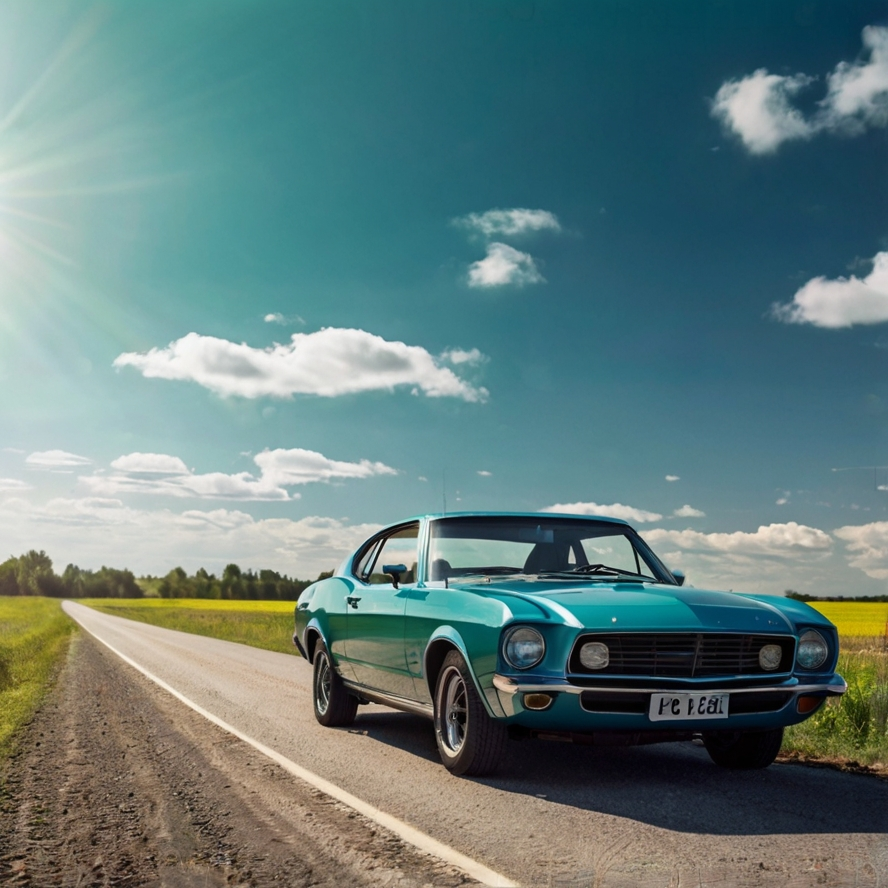
\includegraphics[width=13cm,height=12cm]{tikz/chapter5 - VGGNet.jpg}};
\end{scope}
%-----------------------------------
\node[minimum size=2.5cm] (image) at (-2mm,0) {};
%-----------------------Cubes-------------------------------
\cube{1.5}{0}{}{.25}{6}{6.5}{white}
\cube{1.9}{0}{}{.25}{6}{6.5}{white}

\cube{2.5}{0}{}{.3}{6*.6}{6.5*.6}{mygreen!20}
\cube{2.95}{0}{}{.3}{6*.6}{6.5*.6}{white}
\cube{3.4}{0}{}{.3}{6*.6}{6.5*.6}{white}

\cube{3.8}{0}{}{.37}{6*.3}{6.5*.3}{mygreen!20}
\cube{4.3}{0}{}{.37}{6*.3}{6.5*.3}{white}
\cube{4.8}{0}{}{.37}{6*.3}{6.5*.3}{white}
\cube{5.3}{0}{}{.37}{6*.3}{6.5*.3}{white}

\cube{6}{0}{}{.65}{6*.16}{6.5*.16}{mygreen!20}
\cube{6.8}{0}{}{.65}{6*.16}{6.5*.16}{white}
\cube{7.6}{0}{}{.65}{6*.16}{6.5*.16}{white}
\cube{8.4}{0}{}{.65}{6*.16}{6.5*.16}{white}

\cube{9.2}{0}{}{.65}{6*.08}{6.5*.08}{mygreen!20}
\cube{10}{0}{}{.65}{6*.08}{6.5*.08}{white}
\cube{10.8}{0}{}{.65}{6*.08}{6.5*.08}{white}
\cube{11.6}{0}{}{.65}{6*.08}{6.5*.08}{white}

\cube{12.4}{0}{}{.65}{6*.04}{6.5*.04}{mygreen!20}

\cube{13.3}{0}{}{.95}{6*.02}{6.5*.02}{myblue!15}
\cube{14.35}{0}{}{.95}{6*.02}{6.5*.02}{myblue!15}
\cube{15.25}{0}{}{.65}{6*.02}{6.5*.02}{myblue!15}

\cube{16}{0}{}{.65}{6*.02}{6.5*.02}{myred!20}

% Legend
\cube{12.4}{-2}{}{.4}{6*.04}{6.5*.04}{white}
\cube{12.4}{-2.5}{}{.4}{6*.04}{6.5*.04}{mygreen!20}
\cube{12.4}{-3}{}{.4}{6*.04}{6.5*.04}{myblue!15}
\cube{12.4}{-3.5}{}{.4}{6*.04}{6.5*.04}{myred!20}

\node[anchor=west] at (12.8,-2) {Convolution $+$ ReLU};
\node[anchor=west] at (12.8,-2.5) {Max pooling};
\node[anchor=west] at (12.8,-3) {Fully connected $+$ ReLU};
\node[anchor=west] at (12.8,-3.5) {Softmax};


\node[] at (0.5,4.5) {\rotatebox{0}{$224 \times 224 \times 3$}};
\node[] at (3.7,4.5) {\rotatebox{0}{$224 \times 224 \times 64$}};
\node[] at (4.5,2.8) {\rotatebox{0}{$112 \times 112 \times 128$}};
\node[] at (5.3,1.5) {\rotatebox{0}{$56 \times 56 \times 256$}};
\node[] at (7.5,.9) {\rotatebox{0}{$28 \times 28 \times 512$}};
\node[] at (10.5,.55) {\rotatebox{0}{$14 \times 14 \times 512$}};
\node[] at (13.7,.3) {\rotatebox{0}{$1 \times 1 \times 4096$}};
\node[] at (15.6,-.3) {\rotatebox{0}{$1 \times 1 \times 4096$}};

\draw[<-] (9.2,.4)--node[pos=1,above] {\rotatebox{0}{$7 \times 7 \times 512$}} +(0,1);

}
}

\end{document}
